% Options for packages loaded elsewhere
\PassOptionsToPackage{unicode}{hyperref}
\PassOptionsToPackage{hyphens}{url}
\PassOptionsToPackage{dvipsnames,svgnames,x11names}{xcolor}
%
\documentclass[
  letterpaper,
  DIV=11,
  numbers=noendperiod]{scrartcl}

\usepackage{amsmath,amssymb}
\usepackage{lmodern}
\usepackage{iftex}
\ifPDFTeX
  \usepackage[T1]{fontenc}
  \usepackage[utf8]{inputenc}
  \usepackage{textcomp} % provide euro and other symbols
\else % if luatex or xetex
  \usepackage{unicode-math}
  \defaultfontfeatures{Scale=MatchLowercase}
  \defaultfontfeatures[\rmfamily]{Ligatures=TeX,Scale=1}
\fi
% Use upquote if available, for straight quotes in verbatim environments
\IfFileExists{upquote.sty}{\usepackage{upquote}}{}
\IfFileExists{microtype.sty}{% use microtype if available
  \usepackage[]{microtype}
  \UseMicrotypeSet[protrusion]{basicmath} % disable protrusion for tt fonts
}{}
\makeatletter
\@ifundefined{KOMAClassName}{% if non-KOMA class
  \IfFileExists{parskip.sty}{%
    \usepackage{parskip}
  }{% else
    \setlength{\parindent}{0pt}
    \setlength{\parskip}{6pt plus 2pt minus 1pt}}
}{% if KOMA class
  \KOMAoptions{parskip=half}}
\makeatother
\usepackage{xcolor}
\setlength{\emergencystretch}{3em} % prevent overfull lines
\setcounter{secnumdepth}{-\maxdimen} % remove section numbering
% Make \paragraph and \subparagraph free-standing
\ifx\paragraph\undefined\else
  \let\oldparagraph\paragraph
  \renewcommand{\paragraph}[1]{\oldparagraph{#1}\mbox{}}
\fi
\ifx\subparagraph\undefined\else
  \let\oldsubparagraph\subparagraph
  \renewcommand{\subparagraph}[1]{\oldsubparagraph{#1}\mbox{}}
\fi

\usepackage{color}
\usepackage{fancyvrb}
\newcommand{\VerbBar}{|}
\newcommand{\VERB}{\Verb[commandchars=\\\{\}]}
\DefineVerbatimEnvironment{Highlighting}{Verbatim}{commandchars=\\\{\}}
% Add ',fontsize=\small' for more characters per line
\usepackage{framed}
\definecolor{shadecolor}{RGB}{241,243,245}
\newenvironment{Shaded}{\begin{snugshade}}{\end{snugshade}}
\newcommand{\AlertTok}[1]{\textcolor[rgb]{0.68,0.00,0.00}{#1}}
\newcommand{\AnnotationTok}[1]{\textcolor[rgb]{0.37,0.37,0.37}{#1}}
\newcommand{\AttributeTok}[1]{\textcolor[rgb]{0.40,0.45,0.13}{#1}}
\newcommand{\BaseNTok}[1]{\textcolor[rgb]{0.68,0.00,0.00}{#1}}
\newcommand{\BuiltInTok}[1]{\textcolor[rgb]{0.00,0.23,0.31}{#1}}
\newcommand{\CharTok}[1]{\textcolor[rgb]{0.13,0.47,0.30}{#1}}
\newcommand{\CommentTok}[1]{\textcolor[rgb]{0.37,0.37,0.37}{#1}}
\newcommand{\CommentVarTok}[1]{\textcolor[rgb]{0.37,0.37,0.37}{\textit{#1}}}
\newcommand{\ConstantTok}[1]{\textcolor[rgb]{0.56,0.35,0.01}{#1}}
\newcommand{\ControlFlowTok}[1]{\textcolor[rgb]{0.00,0.23,0.31}{#1}}
\newcommand{\DataTypeTok}[1]{\textcolor[rgb]{0.68,0.00,0.00}{#1}}
\newcommand{\DecValTok}[1]{\textcolor[rgb]{0.68,0.00,0.00}{#1}}
\newcommand{\DocumentationTok}[1]{\textcolor[rgb]{0.37,0.37,0.37}{\textit{#1}}}
\newcommand{\ErrorTok}[1]{\textcolor[rgb]{0.68,0.00,0.00}{#1}}
\newcommand{\ExtensionTok}[1]{\textcolor[rgb]{0.00,0.23,0.31}{#1}}
\newcommand{\FloatTok}[1]{\textcolor[rgb]{0.68,0.00,0.00}{#1}}
\newcommand{\FunctionTok}[1]{\textcolor[rgb]{0.28,0.35,0.67}{#1}}
\newcommand{\ImportTok}[1]{\textcolor[rgb]{0.00,0.46,0.62}{#1}}
\newcommand{\InformationTok}[1]{\textcolor[rgb]{0.37,0.37,0.37}{#1}}
\newcommand{\KeywordTok}[1]{\textcolor[rgb]{0.00,0.23,0.31}{#1}}
\newcommand{\NormalTok}[1]{\textcolor[rgb]{0.00,0.23,0.31}{#1}}
\newcommand{\OperatorTok}[1]{\textcolor[rgb]{0.37,0.37,0.37}{#1}}
\newcommand{\OtherTok}[1]{\textcolor[rgb]{0.00,0.23,0.31}{#1}}
\newcommand{\PreprocessorTok}[1]{\textcolor[rgb]{0.68,0.00,0.00}{#1}}
\newcommand{\RegionMarkerTok}[1]{\textcolor[rgb]{0.00,0.23,0.31}{#1}}
\newcommand{\SpecialCharTok}[1]{\textcolor[rgb]{0.37,0.37,0.37}{#1}}
\newcommand{\SpecialStringTok}[1]{\textcolor[rgb]{0.13,0.47,0.30}{#1}}
\newcommand{\StringTok}[1]{\textcolor[rgb]{0.13,0.47,0.30}{#1}}
\newcommand{\VariableTok}[1]{\textcolor[rgb]{0.07,0.07,0.07}{#1}}
\newcommand{\VerbatimStringTok}[1]{\textcolor[rgb]{0.13,0.47,0.30}{#1}}
\newcommand{\WarningTok}[1]{\textcolor[rgb]{0.37,0.37,0.37}{\textit{#1}}}

\providecommand{\tightlist}{%
  \setlength{\itemsep}{0pt}\setlength{\parskip}{0pt}}\usepackage{longtable,booktabs,array}
\usepackage{calc} % for calculating minipage widths
% Correct order of tables after \paragraph or \subparagraph
\usepackage{etoolbox}
\makeatletter
\patchcmd\longtable{\par}{\if@noskipsec\mbox{}\fi\par}{}{}
\makeatother
% Allow footnotes in longtable head/foot
\IfFileExists{footnotehyper.sty}{\usepackage{footnotehyper}}{\usepackage{footnote}}
\makesavenoteenv{longtable}
\usepackage{graphicx}
\makeatletter
\def\maxwidth{\ifdim\Gin@nat@width>\linewidth\linewidth\else\Gin@nat@width\fi}
\def\maxheight{\ifdim\Gin@nat@height>\textheight\textheight\else\Gin@nat@height\fi}
\makeatother
% Scale images if necessary, so that they will not overflow the page
% margins by default, and it is still possible to overwrite the defaults
% using explicit options in \includegraphics[width, height, ...]{}
\setkeys{Gin}{width=\maxwidth,height=\maxheight,keepaspectratio}
% Set default figure placement to htbp
\makeatletter
\def\fps@figure{htbp}
\makeatother

\KOMAoption{captions}{tableheading}
\makeatletter
\makeatother
\makeatletter
\makeatother
\makeatletter
\@ifpackageloaded{caption}{}{\usepackage{caption}}
\AtBeginDocument{%
\ifdefined\contentsname
  \renewcommand*\contentsname{Table of contents}
\else
  \newcommand\contentsname{Table of contents}
\fi
\ifdefined\listfigurename
  \renewcommand*\listfigurename{List of Figures}
\else
  \newcommand\listfigurename{List of Figures}
\fi
\ifdefined\listtablename
  \renewcommand*\listtablename{List of Tables}
\else
  \newcommand\listtablename{List of Tables}
\fi
\ifdefined\figurename
  \renewcommand*\figurename{Figure}
\else
  \newcommand\figurename{Figure}
\fi
\ifdefined\tablename
  \renewcommand*\tablename{Table}
\else
  \newcommand\tablename{Table}
\fi
}
\@ifpackageloaded{float}{}{\usepackage{float}}
\floatstyle{ruled}
\@ifundefined{c@chapter}{\newfloat{codelisting}{h}{lop}}{\newfloat{codelisting}{h}{lop}[chapter]}
\floatname{codelisting}{Listing}
\newcommand*\listoflistings{\listof{codelisting}{List of Listings}}
\makeatother
\makeatletter
\@ifpackageloaded{caption}{}{\usepackage{caption}}
\@ifpackageloaded{subcaption}{}{\usepackage{subcaption}}
\makeatother
\makeatletter
\@ifpackageloaded{tcolorbox}{}{\usepackage[many]{tcolorbox}}
\makeatother
\makeatletter
\@ifundefined{shadecolor}{\definecolor{shadecolor}{rgb}{.97, .97, .97}}
\makeatother
\makeatletter
\makeatother
\ifLuaTeX
  \usepackage{selnolig}  % disable illegal ligatures
\fi
\IfFileExists{bookmark.sty}{\usepackage{bookmark}}{\usepackage{hyperref}}
\IfFileExists{xurl.sty}{\usepackage{xurl}}{} % add URL line breaks if available
\urlstyle{same} % disable monospaced font for URLs
\hypersetup{
  pdftitle={SENG 474: Assignment 1 Report},
  colorlinks=true,
  linkcolor={blue},
  filecolor={Maroon},
  citecolor={Blue},
  urlcolor={Blue},
  pdfcreator={LaTeX via pandoc}}

\title{SENG 474: Assignment 1 Report}
\usepackage{etoolbox}
\makeatletter
\providecommand{\subtitle}[1]{% add subtitle to \maketitle
  \apptocmd{\@title}{\par {\large #1 \par}}{}{}
}
\makeatother
\subtitle{Nathan Woloshyn}
\author{}
\date{}

\begin{document}
\maketitle
\ifdefined\Shaded\renewenvironment{Shaded}{\begin{tcolorbox}[boxrule=0pt, frame hidden, breakable, interior hidden, sharp corners, enhanced, borderline west={3pt}{0pt}{shadecolor}]}{\end{tcolorbox}}\fi

\hypertarget{part-1-processing-the-data}{%
\subsection{Part 1: Processing the
data}\label{part-1-processing-the-data}}

The first step is to load the data into a pandas dataframe. The data is
stored in a csv file, so we can use the read\_csv function to load it
into a dataframe. After this, we split the data into a training set and
a test set. What fraction of the data is used for training and what
fraction is used for testing is a hyperparameter that can be tuned. We
choose a 75/25 split as our default, but will also analyze the results
of other splits. We also specify a random seed for the sampling, so that
we can reproduce the results of our experiments.

\begin{Shaded}
\begin{Highlighting}[]
\ImportTok{import}\NormalTok{ pandas }\ImportTok{as}\NormalTok{ pd}

\CommentTok{\textquotesingle{}\textquotesingle{}\textquotesingle{}Reads the data from the csv file and returns a pandas dataframe.\textquotesingle{}\textquotesingle{}\textquotesingle{}}
\KeywordTok{def}\NormalTok{ read\_data():}
\NormalTok{    df }\OperatorTok{=}\NormalTok{ pd.read\_csv(}\StringTok{\textquotesingle{}./cleaned\_adult.csv\textquotesingle{}}\NormalTok{)}

    \ControlFlowTok{return}\NormalTok{ df}



\CommentTok{\textquotesingle{}\textquotesingle{}\textquotesingle{}Partitions the data into train and test sets, using a taking what }
\CommentTok{percentage of the data train / test on as input. Returns the train and test\textquotesingle{}\textquotesingle{}\textquotesingle{}}
\KeywordTok{def}\NormalTok{ partition\_data(df, train\_size}\OperatorTok{=}\FloatTok{0.75}\NormalTok{, random\_state}\OperatorTok{=}\DecValTok{99}\NormalTok{):}
    \CommentTok{\# Split the data into train and test sets. (0.75, 0.25) split.}
\NormalTok{    train\_df }\OperatorTok{=}\NormalTok{ df.sample(train\_size, random\_state)}
\NormalTok{    test\_df }\OperatorTok{=}\NormalTok{ df.drop(train\_df.index)}

    \ControlFlowTok{return}\NormalTok{ train\_df, test\_df}

\end{Highlighting}
\end{Shaded}

\hypertarget{part-2-decision-trees}{%
\subsection{Part 2: Decision Trees}\label{part-2-decision-trees}}

\hypertarget{part-2.1-no-pruning}{%
\subsubsection{Part 2.1: No Pruning}\label{part-2.1-no-pruning}}

In our first experiment we use the sklearn implementation of a decision
tree classifier. We use the default parameters, which means that the
tree is not pruned. We use test both entropy and Gini impurity as our
criterion for splitting the tree. Using the code below we test every
depth of tree from 1 to 100 using these two criteria. We use our default
choice of 75/25 train/test split, giving all trees the same train/test
split.

\begin{Shaded}
\begin{Highlighting}[]
\NormalTok{train, test }\OperatorTok{=}\NormalTok{ read\_data.partition\_data(read\_data.read\_data())}


\CommentTok{\textquotesingle{}\textquotesingle{}\textquotesingle{}Test various depths, with entropy as the criterion, }
\CommentTok{store and plot the scores on both training and test sets using matplotlib\textquotesingle{}\textquotesingle{}\textquotesingle{}}
\KeywordTok{def}\NormalTok{ test\_entropy\_depths():}
\NormalTok{    best\_depth }\OperatorTok{=} \DecValTok{0}
\NormalTok{    best\_score }\OperatorTok{=} \DecValTok{0}
\NormalTok{    test\_scores }\OperatorTok{=}\NormalTok{ []}
\NormalTok{    training\_scores }\OperatorTok{=}\NormalTok{ []}
    \ControlFlowTok{for}\NormalTok{ i }\KeywordTok{in} \BuiltInTok{range}\NormalTok{(}\DecValTok{1}\NormalTok{, }\DecValTok{100}\NormalTok{):}
\NormalTok{        eD }\OperatorTok{=}\NormalTok{ DecisionTreeClassifier(random\_state}\OperatorTok{=}\DecValTok{0}\NormalTok{, max\_depth}\OperatorTok{=}\NormalTok{i,}
\NormalTok{         criterion}\OperatorTok{=}\StringTok{"entropy"}\NormalTok{).fit(train.drop(columns}\OperatorTok{=}\NormalTok{[}\StringTok{\textquotesingle{}income\textquotesingle{}}\NormalTok{]), }
\NormalTok{         train[}\StringTok{\textquotesingle{}income\textquotesingle{}}\NormalTok{])}


\NormalTok{        test\_scores.append(eD.score(test.drop(columns}\OperatorTok{=}\NormalTok{[}\StringTok{\textquotesingle{}income\textquotesingle{}}\NormalTok{]), test[}\StringTok{\textquotesingle{}income\textquotesingle{}}\NormalTok{]))}
\NormalTok{        training\_scores.append(eD.score(train.drop(columns}\OperatorTok{=}\NormalTok{[}\StringTok{\textquotesingle{}income\textquotesingle{}}\NormalTok{]), train[}\StringTok{\textquotesingle{}income\textquotesingle{}}\NormalTok{]))}
        \ControlFlowTok{if}\NormalTok{ eD.score(test.drop(columns}\OperatorTok{=}\NormalTok{[}\StringTok{\textquotesingle{}income\textquotesingle{}}\NormalTok{]), test[}\StringTok{\textquotesingle{}income\textquotesingle{}}\NormalTok{]) }\OperatorTok{\textgreater{}}\NormalTok{ best\_score:}
\NormalTok{            best\_score }\OperatorTok{=}\NormalTok{ eD.score(test.drop(columns}\OperatorTok{=}\NormalTok{[}\StringTok{\textquotesingle{}income\textquotesingle{}}\NormalTok{]), test[}\StringTok{\textquotesingle{}income\textquotesingle{}}\NormalTok{])}
\NormalTok{            best\_depth }\OperatorTok{=}\NormalTok{ i}
\NormalTok{    plt.plot(}\BuiltInTok{range}\NormalTok{(}\DecValTok{1}\NormalTok{, }\DecValTok{100}\NormalTok{), test\_scores, label}\OperatorTok{=}\StringTok{\textquotesingle{}Test\textquotesingle{}}\NormalTok{)}
\NormalTok{    plt.plot(}\BuiltInTok{range}\NormalTok{(}\DecValTok{1}\NormalTok{, }\DecValTok{100}\NormalTok{), training\_scores, label}\OperatorTok{=}\StringTok{\textquotesingle{}Training\textquotesingle{}}\NormalTok{)}
\NormalTok{    plt.plot(best\_depth, best\_score, }\StringTok{\textquotesingle{}ro\textquotesingle{}}\NormalTok{, label}\OperatorTok{=}\StringTok{\textquotesingle{}Best score: \textquotesingle{}}
        \OperatorTok{+} \StringTok{"}\SpecialCharTok{\{:.4f\}}\StringTok{"}\NormalTok{.}\BuiltInTok{format}\NormalTok{(best\_score) }\OperatorTok{+} \StringTok{\textquotesingle{} at depth: \textquotesingle{}} \OperatorTok{+} \BuiltInTok{str}\NormalTok{(best\_depth))}
\NormalTok{    plt.legend(loc}\OperatorTok{=}\StringTok{"lower right"}\NormalTok{)}
\NormalTok{    plt.xlabel(}\StringTok{\textquotesingle{}Depth\textquotesingle{}}\NormalTok{)}
\NormalTok{    plt.ylabel(}\StringTok{\textquotesingle{}Score\textquotesingle{}}\NormalTok{)}
\NormalTok{    plt.title(}\StringTok{\textquotesingle{}Entropy, no pruning\textquotesingle{}}\NormalTok{)}
    \CommentTok{\#plt.show()}
\NormalTok{    plt.savefig(}\StringTok{\textquotesingle{}entropy\_no\_pruning\_scores\_varying\_depth.png\textquotesingle{}}\NormalTok{)}
\NormalTok{    plt.clf()}


\CommentTok{\textquotesingle{}\textquotesingle{}\textquotesingle{}Test various depths, with gini as the criterion,}
\CommentTok{store and plot the scores on both the training and test sets using matplotlib\textquotesingle{}\textquotesingle{}\textquotesingle{}}
\KeywordTok{def}\NormalTok{ test\_gini\_depths():}
\NormalTok{    best\_depth }\OperatorTok{=} \DecValTok{0}
\NormalTok{    best\_score }\OperatorTok{=} \DecValTok{0}
\NormalTok{    test\_scores }\OperatorTok{=}\NormalTok{ []}
\NormalTok{    training\_scores }\OperatorTok{=}\NormalTok{ []}
    \ControlFlowTok{for}\NormalTok{ i }\KeywordTok{in} \BuiltInTok{range}\NormalTok{(}\DecValTok{1}\NormalTok{, }\DecValTok{100}\NormalTok{):}
\NormalTok{        gD }\OperatorTok{=}\NormalTok{ DecisionTreeClassifier(random\_state}\OperatorTok{=}\DecValTok{0}\NormalTok{, max\_depth}\OperatorTok{=}\NormalTok{i, }
\NormalTok{        criterion}\OperatorTok{=}\StringTok{"gini"}\NormalTok{).fit(train.drop(columns}\OperatorTok{=}\NormalTok{[}\StringTok{\textquotesingle{}income\textquotesingle{}}\NormalTok{]), train[}\StringTok{\textquotesingle{}income\textquotesingle{}}\NormalTok{])}
        
\NormalTok{        test\_scores.append(gD.score(test.drop(columns}\OperatorTok{=}\NormalTok{[}\StringTok{\textquotesingle{}income\textquotesingle{}}\NormalTok{]), test[}\StringTok{\textquotesingle{}income\textquotesingle{}}\NormalTok{]))}
\NormalTok{        training\_scores.append(gD.score(train.drop(columns}\OperatorTok{=}\NormalTok{[}\StringTok{\textquotesingle{}income\textquotesingle{}}\NormalTok{]), train[}\StringTok{\textquotesingle{}income\textquotesingle{}}\NormalTok{]))}
        \ControlFlowTok{if}\NormalTok{ gD.score(test.drop(columns}\OperatorTok{=}\NormalTok{[}\StringTok{\textquotesingle{}income\textquotesingle{}}\NormalTok{]), test[}\StringTok{\textquotesingle{}income\textquotesingle{}}\NormalTok{]) }\OperatorTok{\textgreater{}}\NormalTok{ best\_score:}
\NormalTok{            best\_score }\OperatorTok{=}\NormalTok{ gD.score(test.drop(columns}\OperatorTok{=}\NormalTok{[}\StringTok{\textquotesingle{}income\textquotesingle{}}\NormalTok{]), test[}\StringTok{\textquotesingle{}income\textquotesingle{}}\NormalTok{])}
\NormalTok{            best\_depth }\OperatorTok{=}\NormalTok{ i}
\NormalTok{    plt.plot(}\BuiltInTok{range}\NormalTok{(}\DecValTok{1}\NormalTok{, }\DecValTok{100}\NormalTok{), test\_scores, label}\OperatorTok{=}\StringTok{\textquotesingle{}Test\textquotesingle{}}\NormalTok{)}
\NormalTok{    plt.plot(}\BuiltInTok{range}\NormalTok{(}\DecValTok{1}\NormalTok{, }\DecValTok{100}\NormalTok{), training\_scores, label}\OperatorTok{=}\StringTok{\textquotesingle{}Training\textquotesingle{}}\NormalTok{)}
\NormalTok{    plt.plot(best\_depth, best\_score, }\StringTok{\textquotesingle{}ro\textquotesingle{}}\NormalTok{, label}\OperatorTok{=}\StringTok{\textquotesingle{}Best score: \textquotesingle{}}
         \OperatorTok{+} \StringTok{"}\SpecialCharTok{\{:.4f\}}\StringTok{"}\NormalTok{.}\BuiltInTok{format}\NormalTok{(best\_score) }\OperatorTok{+} \StringTok{\textquotesingle{} at depth: \textquotesingle{}} \OperatorTok{+} \BuiltInTok{str}\NormalTok{(best\_depth))}
\NormalTok{    plt.legend(loc}\OperatorTok{=}\StringTok{"lower right"}\NormalTok{)}
\NormalTok{    plt.xlabel(}\StringTok{\textquotesingle{}Depth\textquotesingle{}}\NormalTok{)}
\NormalTok{    plt.ylabel(}\StringTok{\textquotesingle{}Score\textquotesingle{}}\NormalTok{)}
\NormalTok{    plt.title(}\StringTok{\textquotesingle{}Gini, no pruning\textquotesingle{}}\NormalTok{)}
    \CommentTok{\#plt.show()}
\NormalTok{    plt.savefig(}\StringTok{\textquotesingle{}gini\_no\_pruning\_scores\_varying\_depth.png\textquotesingle{}}\NormalTok{)}
\NormalTok{    plt.clf()}

\NormalTok{test\_entropy\_depths()}
\NormalTok{test\_gini\_depths()}
\end{Highlighting}
\end{Shaded}

Running the code above gives us the following results:

\newpage{}

\begin{figure}

\begin{minipage}[t]{0.50\linewidth}

{\centering 

\raisebox{-\height}{

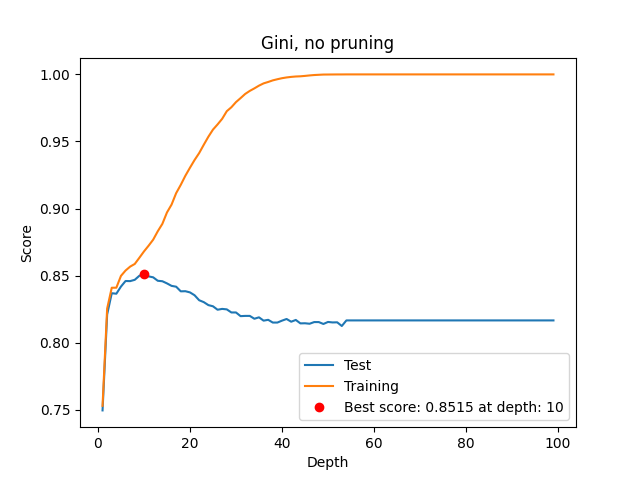
\includegraphics{figures/dt_gini_no_pruning_scores_varying_depth.png}

}

}

\end{minipage}%
%
\begin{minipage}[t]{0.50\linewidth}

{\centering 

\raisebox{-\height}{

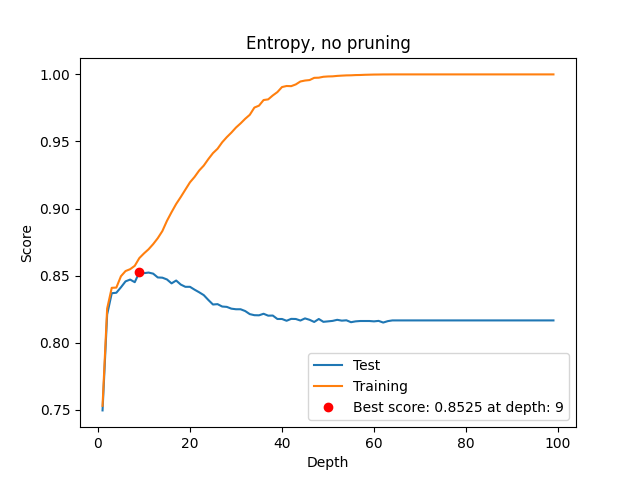
\includegraphics{figures/dt_entropy_no_pruning_scores_varying_depth.png}

}

}

\end{minipage}%

\end{figure}

We can see that at low depth accuracy quickly grows as we allow a tree
to make more splits, but around depth = 10 the models performance
quickly declines. This is likely due to overfitting, as we can see that
as depth increases the training accuracy continues to increase, but the
test accuracy starts to decrease. This is a sign that the model is
overfitting to the training data, and is not generalizing well to the
test data. This is a common problem with decision trees, and why we will
be using pruning in our next experiment. Overall, the two choices of
criterion, entropy and Gini impurity, seem to perform similarly, with
the best score being around 0.85 for both, and both having a best depth
of around 10.

Next we test the effect of varying what percentage of the data we
allocate to training and test, using the same depth of 10 for the tree.
We use the code below to test the effect of varying the train/test split
from 0\% to 100\% in 1\% increments.

\begin{Shaded}
\begin{Highlighting}[]
\CommentTok{\textquotesingle{}\textquotesingle{}\textquotesingle{}Test various training set sizes, with entropy as the criterion, using depth = 10\textquotesingle{}\textquotesingle{}\textquotesingle{}}

\KeywordTok{def}\NormalTok{ test\_entropy\_sizes():}
\NormalTok{    best\_size }\OperatorTok{=} \DecValTok{0}
\NormalTok{    best\_score }\OperatorTok{=} \DecValTok{0}
\NormalTok{    test\_scores }\OperatorTok{=}\NormalTok{ []}
\NormalTok{    training\_scores }\OperatorTok{=}\NormalTok{ []}
    \ControlFlowTok{for}\NormalTok{ i }\KeywordTok{in} \BuiltInTok{range}\NormalTok{(}\DecValTok{1}\NormalTok{, }\DecValTok{100}\NormalTok{):}
\NormalTok{        train, test }\OperatorTok{=}\NormalTok{ read\_data.partition\_data(read\_data.read\_data(), train\_size}\OperatorTok{=}\NormalTok{i}\OperatorTok{/}\DecValTok{100}\NormalTok{)}
\NormalTok{        eS }\OperatorTok{=}\NormalTok{ DecisionTreeClassifier(random\_state}\OperatorTok{=}\DecValTok{0}\NormalTok{, max\_depth}\OperatorTok{=}\DecValTok{10}\NormalTok{, }
\NormalTok{            criterion}\OperatorTok{=}\StringTok{"entropy"}\NormalTok{).fit(train.drop(columns}\OperatorTok{=}\NormalTok{[}\StringTok{\textquotesingle{}income\textquotesingle{}}\NormalTok{]), train[}\StringTok{\textquotesingle{}income\textquotesingle{}}\NormalTok{])}
\NormalTok{        test\_scores.append(eS.score(test.drop(columns}\OperatorTok{=}\NormalTok{[}\StringTok{\textquotesingle{}income\textquotesingle{}}\NormalTok{]), test[}\StringTok{\textquotesingle{}income\textquotesingle{}}\NormalTok{]))}
\NormalTok{        training\_scores.append(eS.score(train.drop(columns}\OperatorTok{=}\NormalTok{[}\StringTok{\textquotesingle{}income\textquotesingle{}}\NormalTok{]), train[}\StringTok{\textquotesingle{}income\textquotesingle{}}\NormalTok{]))}
        \ControlFlowTok{if}\NormalTok{ eS.score(test.drop(columns}\OperatorTok{=}\NormalTok{[}\StringTok{\textquotesingle{}income\textquotesingle{}}\NormalTok{]), test[}\StringTok{\textquotesingle{}income\textquotesingle{}}\NormalTok{]) }\OperatorTok{\textgreater{}}\NormalTok{ best\_score:}
\NormalTok{            best\_score }\OperatorTok{=}\NormalTok{ eS.score(test.drop(columns}\OperatorTok{=}\NormalTok{[}\StringTok{\textquotesingle{}income\textquotesingle{}}\NormalTok{]), test[}\StringTok{\textquotesingle{}income\textquotesingle{}}\NormalTok{])}
\NormalTok{            best\_size }\OperatorTok{=}\NormalTok{ i}
\NormalTok{    plt.plot(}\BuiltInTok{range}\NormalTok{(}\DecValTok{1}\NormalTok{, }\DecValTok{100}\NormalTok{), test\_scores, label}\OperatorTok{=}\StringTok{\textquotesingle{}Test\textquotesingle{}}\NormalTok{)}
\NormalTok{    plt.plot(}\BuiltInTok{range}\NormalTok{(}\DecValTok{1}\NormalTok{, }\DecValTok{100}\NormalTok{), training\_scores, label}\OperatorTok{=}\StringTok{\textquotesingle{}Training\textquotesingle{}}\NormalTok{)}
\NormalTok{    plt.plot(best\_size, best\_score, }\StringTok{\textquotesingle{}ro\textquotesingle{}}\NormalTok{, label}\OperatorTok{=}\StringTok{\textquotesingle{}Best score: \textquotesingle{}}
         \OperatorTok{+} \StringTok{"}\SpecialCharTok{\{:.4f\}}\StringTok{"}\NormalTok{.}\BuiltInTok{format}\NormalTok{(best\_score) }\OperatorTok{+} \StringTok{\textquotesingle{} at size: \textquotesingle{}} \OperatorTok{+} \BuiltInTok{str}\NormalTok{(best\_size))}
\NormalTok{    plt.legend(loc}\OperatorTok{=}\StringTok{"lower right"}\NormalTok{)}
\NormalTok{    plt.xlabel(}\StringTok{\textquotesingle{}Size\textquotesingle{}}\NormalTok{)}
\NormalTok{    plt.ylabel(}\StringTok{\textquotesingle{}Score\textquotesingle{}}\NormalTok{)}
\NormalTok{    plt.title(}\StringTok{\textquotesingle{}Entropy, no pruning\textquotesingle{}}\NormalTok{)}
    \CommentTok{\#plt.show()}
\NormalTok{    plt.savefig(}\StringTok{\textquotesingle{}entropy\_no\_pruning\_scores\_varying\_size.png\textquotesingle{}}\NormalTok{)}
\NormalTok{    plt.clf()}

\CommentTok{\textquotesingle{}\textquotesingle{}\textquotesingle{}Test various training set sizes, with gini as the criterion, using depth = 10\textquotesingle{}\textquotesingle{}\textquotesingle{}}

\KeywordTok{def}\NormalTok{ test\_gini\_sizes():}
\NormalTok{    best\_size }\OperatorTok{=} \DecValTok{0}
\NormalTok{    best\_score }\OperatorTok{=} \DecValTok{0}
\NormalTok{    test\_scores }\OperatorTok{=}\NormalTok{ []}
\NormalTok{    training\_scores }\OperatorTok{=}\NormalTok{ []}
    \ControlFlowTok{for}\NormalTok{ i }\KeywordTok{in} \BuiltInTok{range}\NormalTok{(}\DecValTok{1}\NormalTok{, }\DecValTok{100}\NormalTok{):}
\NormalTok{        train, test }\OperatorTok{=}\NormalTok{ read\_data.partition\_data(read\_data.read\_data(), train\_size}\OperatorTok{=}\NormalTok{i}\OperatorTok{/}\DecValTok{100}\NormalTok{)}
\NormalTok{        gS }\OperatorTok{=}\NormalTok{ DecisionTreeClassifier(random\_state}\OperatorTok{=}\DecValTok{0}\NormalTok{, max\_depth}\OperatorTok{=}\DecValTok{10}\NormalTok{, }
\NormalTok{            criterion}\OperatorTok{=}\StringTok{"gini"}\NormalTok{).fit(train.drop(columns}\OperatorTok{=}\NormalTok{[}\StringTok{\textquotesingle{}income\textquotesingle{}}\NormalTok{]), train[}\StringTok{\textquotesingle{}income\textquotesingle{}}\NormalTok{])}
\NormalTok{        test\_scores.append(gS.score(test.drop(columns}\OperatorTok{=}\NormalTok{[}\StringTok{\textquotesingle{}income\textquotesingle{}}\NormalTok{]), test[}\StringTok{\textquotesingle{}income\textquotesingle{}}\NormalTok{]))}
\NormalTok{        training\_scores.append(gS.score(train.drop(columns}\OperatorTok{=}\NormalTok{[}\StringTok{\textquotesingle{}income\textquotesingle{}}\NormalTok{]), train[}\StringTok{\textquotesingle{}income\textquotesingle{}}\NormalTok{]))}
        \ControlFlowTok{if}\NormalTok{ gS.score(test.drop(columns}\OperatorTok{=}\NormalTok{[}\StringTok{\textquotesingle{}income\textquotesingle{}}\NormalTok{]), test[}\StringTok{\textquotesingle{}income\textquotesingle{}}\NormalTok{]) }\OperatorTok{\textgreater{}}\NormalTok{ best\_score:}
\NormalTok{            best\_score }\OperatorTok{=}\NormalTok{ gS.score(test.drop(columns}\OperatorTok{=}\NormalTok{[}\StringTok{\textquotesingle{}income\textquotesingle{}}\NormalTok{]), test[}\StringTok{\textquotesingle{}income\textquotesingle{}}\NormalTok{])}
\NormalTok{            best\_size }\OperatorTok{=}\NormalTok{ i}
\NormalTok{    plt.plot(}\BuiltInTok{range}\NormalTok{(}\DecValTok{1}\NormalTok{, }\DecValTok{100}\NormalTok{), test\_scores, label}\OperatorTok{=}\StringTok{\textquotesingle{}Test\textquotesingle{}}\NormalTok{)}
\NormalTok{    plt.plot(}\BuiltInTok{range}\NormalTok{(}\DecValTok{1}\NormalTok{, }\DecValTok{100}\NormalTok{), training\_scores, label}\OperatorTok{=}\StringTok{\textquotesingle{}Training\textquotesingle{}}\NormalTok{)}
\NormalTok{    plt.plot(best\_size, best\_score, }\StringTok{\textquotesingle{}ro\textquotesingle{}}\NormalTok{, label}\OperatorTok{=}\StringTok{\textquotesingle{}Best score: \textquotesingle{}} 
        \OperatorTok{+} \StringTok{"}\SpecialCharTok{\{:.4f\}}\StringTok{"}\NormalTok{.}\BuiltInTok{format}\NormalTok{(best\_score) }\OperatorTok{+} \StringTok{\textquotesingle{} at size: \textquotesingle{}} \OperatorTok{+} \BuiltInTok{str}\NormalTok{(best\_size))}
\NormalTok{    plt.legend(loc}\OperatorTok{=}\StringTok{"lower right"}\NormalTok{)}
\NormalTok{    plt.xlabel(}\StringTok{\textquotesingle{}Size\textquotesingle{}}\NormalTok{)}
\NormalTok{    plt.ylabel(}\StringTok{\textquotesingle{}Score\textquotesingle{}}\NormalTok{)}
\NormalTok{    plt.title(}\StringTok{\textquotesingle{}Gini, no pruning\textquotesingle{}}\NormalTok{)}
    \CommentTok{\#plt.show()}
\NormalTok{    plt.savefig(}\StringTok{\textquotesingle{}gini\_no\_pruning\_scores\_varying\_size.png\textquotesingle{}}\NormalTok{)}
\NormalTok{    plt.clf()}

\NormalTok{test\_entropy\_sizes()}
\NormalTok{test\_gini\_sizes()}
\end{Highlighting}
\end{Shaded}

Running the code above gives us the following results:

\begin{figure}

\begin{minipage}[t]{0.50\linewidth}

{\centering 

\raisebox{-\height}{

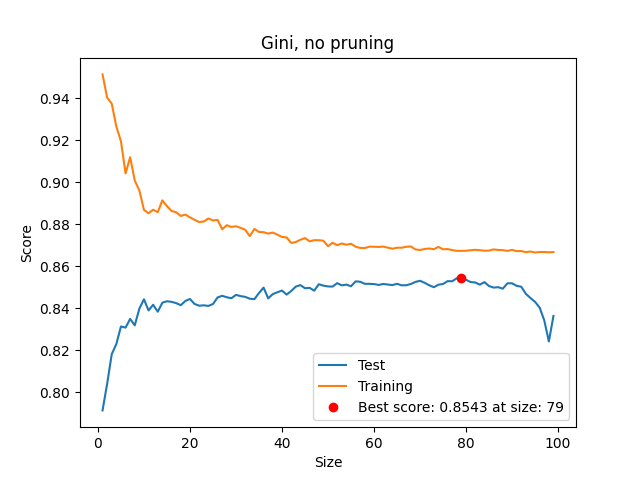
\includegraphics{figures/dt_gini_no_pruning_scores_varying_size.png}

}

}

\end{minipage}%
%
\begin{minipage}[t]{0.50\linewidth}

{\centering 

\raisebox{-\height}{

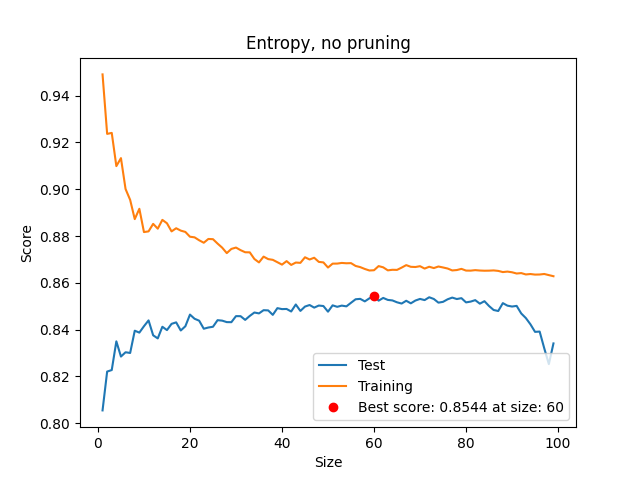
\includegraphics{figures/dt_entropy_no_pruning_scores_varying_size.png}

}

}

\end{minipage}%

\end{figure}

We can see that the accuracy of of the model is sensitive to how we
partition our data. As we increase the size of the training set, the
accuracy of the model increases, but at some point the accuracy the
returns become diminishing, and eventually the test set is so small that
the model is not able to generalize well. However, unlike the last
experiment, there seems to be meaningfully different behavior from our
two criteria. We were surprised by this, given the first experiment. So
we ran several trials of this experiment, varying the random seed used
to partition the data, and the results were consistent. The Gini
criterion sees it's best performance when around 80\% of the data is
allocated to training, while the entropy criterion consistently reaches
peak performance when around 60\% of the data is allocated to training.

\hypertarget{part-2.2-pruning}{%
\subsubsection{Part 2.2: Pruning}\label{part-2.2-pruning}}

Now we will introduce pruning to our decision trees. We will be
performing similar experiments with varying depth and varying training
set size, but this time we will be using the pruning parameter to
control the depth of the tree. We will be using the same methodology as
before, but with the addition of the pruning parameter. Similar to our
previous experiment, we will test the effect varying the pruning
parameter \[ \alpha \] through all possible values and observing the
effect on the accuracy of the model. We will be using the entropy
criterion for this experiment, and the same training set size of 75\%
for the data.

\begin{Shaded}
\begin{Highlighting}[]


\NormalTok{train, test }\OperatorTok{=}\NormalTok{ read\_data.partition\_data(read\_data.read\_data())}


\CommentTok{\#create dt}
\NormalTok{dt }\OperatorTok{=}\NormalTok{ DecisionTreeClassifier(random\_state}\OperatorTok{=}\DecValTok{0}\NormalTok{, criterion}\OperatorTok{=}\StringTok{"entropy"}\NormalTok{).fit(train.drop(columns}\OperatorTok{=}\NormalTok{[}\StringTok{\textquotesingle{}income\textquotesingle{}}\NormalTok{]), train[}\StringTok{\textquotesingle{}income\textquotesingle{}}\NormalTok{])}

\CommentTok{\#prune dt}
\NormalTok{path }\OperatorTok{=}\NormalTok{ dt.cost\_complexity\_pruning\_path(train.drop(columns}\OperatorTok{=}\NormalTok{[}\StringTok{\textquotesingle{}income\textquotesingle{}}\NormalTok{]), train[}\StringTok{\textquotesingle{}income\textquotesingle{}}\NormalTok{])}
\NormalTok{ccp\_alphas, impurities }\OperatorTok{=}\NormalTok{ path.ccp\_alphas, path.impurities}

\NormalTok{depths }\OperatorTok{=}\NormalTok{ []}
\NormalTok{scores }\OperatorTok{=}\NormalTok{ []}
\NormalTok{i }\OperatorTok{=} \DecValTok{0}
\NormalTok{best\_alpha }\OperatorTok{=}\NormalTok{ ccp\_alphas[}\DecValTok{0}\NormalTok{]}
\NormalTok{best\_score }\OperatorTok{=} \DecValTok{0}
\ControlFlowTok{for}\NormalTok{ ccp\_alpha }\KeywordTok{in}\NormalTok{ ccp\_alphas:}
    \ControlFlowTok{if}\NormalTok{ i }\OperatorTok{\%} \DecValTok{100} \OperatorTok{==} \DecValTok{0}\NormalTok{:}
        \BuiltInTok{print}\NormalTok{(i)}
\NormalTok{    dt\_pruned }\OperatorTok{=}\NormalTok{ DecisionTreeClassifier(random\_state}\OperatorTok{=}\DecValTok{0}\NormalTok{, criterion}\OperatorTok{=}\StringTok{"entropy"}\NormalTok{, ccp\_alpha}\OperatorTok{=}\NormalTok{ccp\_alpha).fit(train.drop(columns}\OperatorTok{=}\NormalTok{[}\StringTok{\textquotesingle{}income\textquotesingle{}}\NormalTok{]), train[}\StringTok{\textquotesingle{}income\textquotesingle{}}\NormalTok{])}
    \ControlFlowTok{if}\NormalTok{ dt\_pruned.score(test.drop(columns}\OperatorTok{=}\NormalTok{[}\StringTok{\textquotesingle{}income\textquotesingle{}}\NormalTok{]), test[}\StringTok{\textquotesingle{}income\textquotesingle{}}\NormalTok{]) }\OperatorTok{\textgreater{}}\NormalTok{ best\_score:}
\NormalTok{            best\_score }\OperatorTok{=}\NormalTok{ dt\_pruned.score(test.drop(columns}\OperatorTok{=}\NormalTok{[}\StringTok{\textquotesingle{}income\textquotesingle{}}\NormalTok{]), test[}\StringTok{\textquotesingle{}income\textquotesingle{}}\NormalTok{])}
\NormalTok{            best\_alpha }\OperatorTok{=}\NormalTok{ ccp\_alpha}
\NormalTok{    depths.append(dt\_pruned.get\_depth())}
\NormalTok{    scores.append(dt\_pruned.score(test.drop(columns}\OperatorTok{=}\NormalTok{[}\StringTok{\textquotesingle{}income\textquotesingle{}}\NormalTok{]), test[}\StringTok{\textquotesingle{}income\textquotesingle{}}\NormalTok{]))}
\NormalTok{    i}\OperatorTok{+=}\DecValTok{1}

\CommentTok{\textquotesingle{}\textquotesingle{}\textquotesingle{}Plot the scores on both the training and test sets using matplotlib from varying alpha values\textquotesingle{}\textquotesingle{}\textquotesingle{}}

\KeywordTok{def}\NormalTok{ plot\_alpha\_scores():}
\NormalTok{    plt.plot(ccp\_alphas, scores, label}\OperatorTok{=}\StringTok{\textquotesingle{}Scores\textquotesingle{}}\NormalTok{)}
\NormalTok{    plt.plot(best\_alpha, best\_score, }\StringTok{\textquotesingle{}ro\textquotesingle{}}\NormalTok{, label}\OperatorTok{=}\StringTok{\textquotesingle{}Best score: \textquotesingle{}}
        \OperatorTok{+} \StringTok{"}\SpecialCharTok{\{:.4f\}}\StringTok{"}\NormalTok{.}\BuiltInTok{format}\NormalTok{(best\_score) }\OperatorTok{+} \StringTok{\textquotesingle{} at alpha: \textquotesingle{}} \OperatorTok{+} \BuiltInTok{str}\NormalTok{(best\_alpha))}
\NormalTok{    plt.legend(loc}\OperatorTok{=}\StringTok{"upper right"}\NormalTok{)}
\NormalTok{    plt.xlabel(}\StringTok{\textquotesingle{}Alpha\textquotesingle{}}\NormalTok{)}
\NormalTok{    plt.ylabel(}\StringTok{\textquotesingle{}Score\textquotesingle{}}\NormalTok{)}
\NormalTok{    plt.title(}\StringTok{\textquotesingle{}Entropy, pruning\textquotesingle{}}\NormalTok{)}
\NormalTok{    plt.savefig(}\StringTok{\textquotesingle{}entropy\_pruning\_scores\_varying\_alpha.png\textquotesingle{}}\NormalTok{)}
\NormalTok{    plt.clf()}

\CommentTok{\textquotesingle{}\textquotesingle{}\textquotesingle{}plot the depths as alpha varies\textquotesingle{}\textquotesingle{}\textquotesingle{}}
\KeywordTok{def}\NormalTok{ plot\_alpha\_depths():}
\NormalTok{    plt.plot(ccp\_alphas, depths, label}\OperatorTok{=}\StringTok{\textquotesingle{}Depth\textquotesingle{}}\NormalTok{)}
\NormalTok{    plt.legend(loc}\OperatorTok{=}\StringTok{"upper right"}\NormalTok{)}
\NormalTok{    plt.xlabel(}\StringTok{\textquotesingle{}Alpha\textquotesingle{}}\NormalTok{)}
\NormalTok{    plt.ylabel(}\StringTok{\textquotesingle{}Depth\textquotesingle{}}\NormalTok{)}
\NormalTok{    plt.title(}\StringTok{\textquotesingle{}Entropy, pruning\textquotesingle{}}\NormalTok{)}
\NormalTok{    plt.savefig(}\StringTok{\textquotesingle{}entropy\_pruning\_depths\_varying\_alpha.png\textquotesingle{}}\NormalTok{)}
\NormalTok{    plt.clf()}

\NormalTok{plot\_alpha\_scores()}
\NormalTok{plot\_alpha\_depths()}
\end{Highlighting}
\end{Shaded}

This code lets a decision tree grow to full depth, and then we collect
all the possible cost complexity pruning paths and their alpha values.
Then we create a tree with each value and measure its score on the test
set, we also record the max depth of each such tree. We can see the
results below:

\begin{figure}

\begin{minipage}[t]{0.50\linewidth}

{\centering 

\raisebox{-\height}{

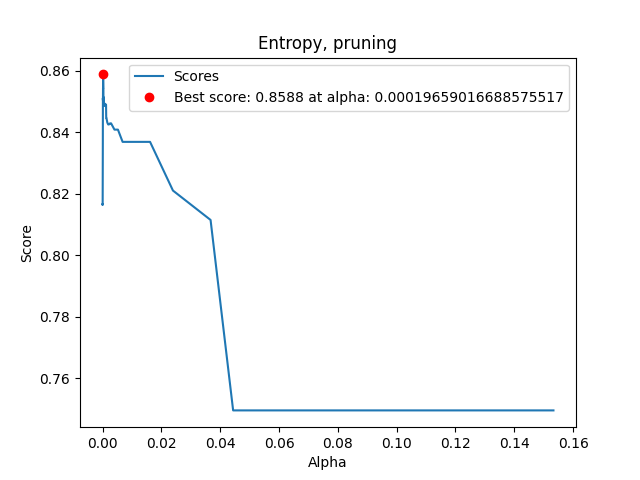
\includegraphics{figures/dt_entropy_pruning_scores_varying_alpha.png}

}

}

\end{minipage}%
%
\begin{minipage}[t]{0.50\linewidth}

{\centering 

\raisebox{-\height}{

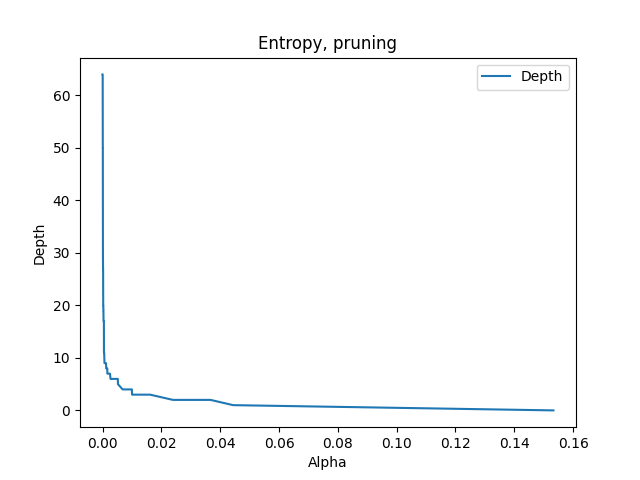
\includegraphics{figures/dt_entropy_pruning_depths_varying_alpha.png}

}

}

\end{minipage}%

\end{figure}

We can see that with a well chosen \(\alpha\) we get a small but
noticeable improvement over our best score in the non pruning
experiments (0.86 vs 0.85). A one percent improvement might seem very
small, but considering that the classification rate is already somewhat
high, the absolute number of errors lower by a factor of
\(\frac{1}{15}\).

\hypertarget{part-3-random-forests}{%
\subsubsection{Part 3: Random Forests}\label{part-3-random-forests}}



\end{document}
